\section{Boundary layer}
To introduce the concept of a boundary layer, one has to think of a uniform flow
in one direction with a certain speed ($U_{\infty}$). Now place a thin plate
into this flow where its long side aligns with the flow direction. This setup is
know as \textit{flat plate at zero incidence}. At the surface of the wall, the
\textit{no slip condition} must be satisfied. This means, the flow slows down
until it reaches exactly zero at the surface. This slow down does not happen
linearly and a large portion of the flow remains uniform. The flow is slowed
down only near the surface of the plate due to friction forces. This area is
called the \textit{boundary layer} or \textit{frictional layer}. It's thickness
($\delta(x)$) depends on a lot of different factors, but most prominently on its
position from the leading edge. In reality, there is no hard border between the
uniform flow and the boundary layer. Thus it is often defined as where the flow
reaches 99\% of the velocity of the outer flow \cite{Schlichting2018}. Figure
\ref{fig:boundary_layer_flat_plate} shows this concept.

\begin{figure}[H] \centering
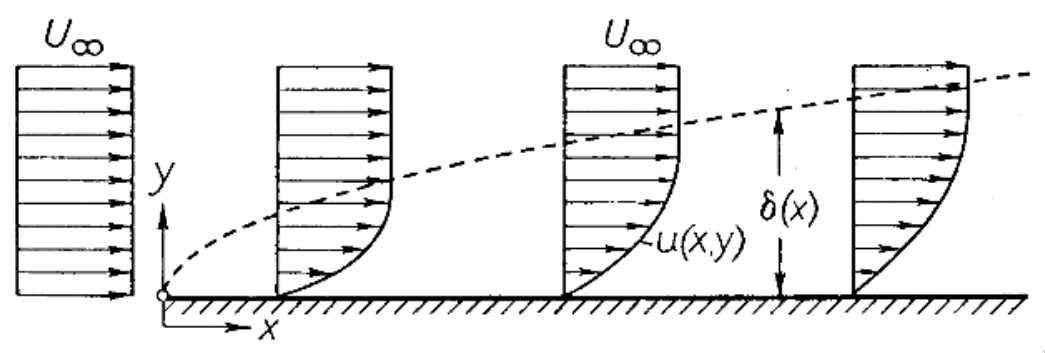
\includegraphics[width=0.5\textwidth]{boundary_layer_flat_plate}
    \caption{Laminar boundary layer of a flat plate at zero incidence \cite{Schlichting2018}.}
    \label{fig:boundary_layer_flat_plate}
\end{figure}

\paragraph{Types of boundary layers}
The flow inside the boundary layer might be \textit{laminar} or
\textit{turbulent}. In reality, it is laminar at the leading edge, transitions
to turbulence over a certain length and becomes fully turbulent afterwards
\cite{Schlichting2018}. As this report deals with a fully turbulent
\textit{turbulence model}, the first two types of boundary layer are not
explained further.

\paragraph{Frictional forces}
As explained earlier, the flow in the boundary layer is slowed down until it
becomes zero at the surface. This slowing down exerts a force in the flow
direction on the surface. This force, normalized by its application area, is
called \textit{shear stress} ($\tau_{w}$). To obtain a dimensionless
coefficient, which may be easily compared, the shear stress is divided by the
\textit{dynamic pressure} \cite{Schlichting2018}:

\begin{equation}
  c_{f} = \frac{\tau_{w}(x)}{\frac{1}{2}\rho U_{\infty}^{2}}
\end{equation}

\noindent Where $\rho$ is the density of the fluid.


\subsection{Turbulent boundary layer}
\label{sec:turbulent_BL}
When looking closer at a turbulent boundary layer, once can observer two
different regions. At the top is a \textit{turbulent layer} which is only
indirectly affected by the friction with the wall. At the bottom is a layer that
is really thin compared to the boundary layer. It is called \textit{viscous
sublayer} or \textit{viscous wall layer} and is directly affected by the
friction. As is the case with the boundary layer itself, there is no hard border
between those two regions. Instead one can observe a smooth transition
\cite{Schlichting2018}.

To examine the cross section of the boundary layer, it make sens to introduce
the concept of the dimensionless \textit{wall distance} $y^{+}$. Hand in hand
goes the dimensionless velocity $u^{+}$. Moving to this dimensionless system
allows us to compare different boundary layers from different flow conditions
more easily. The velocity $u^{+}$ is given by \cite{Schlichting2018}:

\begin{equation}
  u^{+} = \frac{u}{u_{\tau}}
\end{equation}

\noindent Where as $u$ is the flow velocity and $u_{\tau}$ the \textit{friction velocity}.
It is given by:

\begin{equation}
  u_{\tau} = \sqrt{\frac{\tau_{w}}{\rho}}
\end{equation}

\noindent As before, $\tau_{w}$ is the \textit{shear stress} and $\rho$ the
\textit{density}. The dimensionless \textit{wall distance} $y^{+}$ is given by:

\begin{equation}
  y^{+} = \frac{yu_{\tau}}{\nu}
\end{equation}

\noindent Where as $y$ is the distance to the wall and $\nu$ is the \textit{kinematic
viscosity} of the fluid.


\subsubsection{Universal law of the wall}
Theory which describes the velocity distribution of a turbulent boundary layer
in fully developed flow\footnote{This means, the flow does not change with
increasing x.}  is know as the \textit{universal law of the wall}. It defines the
different regions as follows \cite{Schlichting2018}:

\paragraph{Viscous sublayer ($y^{+} < 5$)}
For the viscous sublayer, $u^{+}$ is given by:

\begin{equation}
  u^{+} = y^{+}
\end{equation}

\paragraph{Logarithmic overlap law ($y^{+} > 30$)}
In the fully turbulent region at the top of the boundary layer, the turbulence
stress dominates and the velocity profile varies very slowly with a logarithmic
function:

\begin{equation}
  u^{+} = \frac{1}{\kappa} ln(y^{+}) + C^{+}
  \label{eq:overlap_law}
\end{equation}

\noindent The Karman constant $\kappa$ is equal to $0.41$ and $C^{+}$ equals to
$5.0$ for smooth walls.

\paragraph{Overlap layer ($5 < y^{+} < 30$)}
The \textit{overlap layer} is located between the viscous sublayer and the
logarithmic area. It is a region where the flow transitions from one to the
other. It can not be described with such an easy equation as for the other two
regions.

If we plot the wall distance $y^{+}$ on a logarithmic scale and the velocity
$u^{+}$ on a linear scale, the different regions are obvious. Take a look at
figure \ref{fig:law_of_wall}.

\begin{figure}[H] \centering
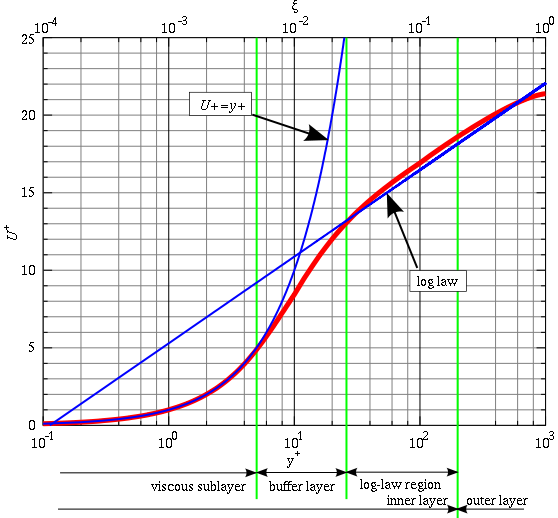
\includegraphics[width=0.45\textwidth]{law_of_wall}
    \caption{Cross section of a fully developed turbulent boundary layer
             overlayed with measurements\cite{Schlichting2018}.}
    \label{fig:law_of_wall}
\end{figure}





\subsection{The effect of roughness}
\label{subsec:roughness}
Before the effects of roughness may be investigated, it makes sense to describe
a standard roughness which is easier to compare. Take a look at figure
\ref{fig:sand_roughness}. It is assumed the surface is tightly packed with balls
of equal diameter. Because this is similar to sandpaper, this roughness is
called \textit{sand roughness} or \textit{standard roughness}. The diameter of
the balls is the \textit{sand roughness height} $k_{s}$. It is a measure for the
roughness of a surface \cite{Schlichting2018}.

\begin{figure}[H] \centering
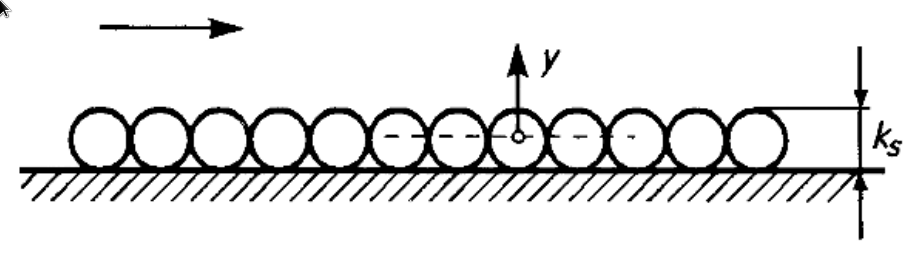
\includegraphics[width=0.45\textwidth]{sand_roughness}
    \caption{Definition of \textit{sand roughness} and $k_{s}$ \cite{Schlichting2018}.}
    \label{fig:sand_roughness}
\end{figure}

\noindent Analog to $u^{+}$ and $y^{+}$ (see section \ref{sec:turbulent_BL}),
there exists a dimensionless $k_{s}^{+}$:

\begin{equation}
  k_{s}^{+} = \frac{k_{s}u_{\tau}}{\nu}
\end{equation}

\paragraph{Equivalent sand roughness}
Real surfaces are not made up of balls as assumed in figure
\ref{fig:sand_roughness}, but instead have a random distribution of peaks and
vales. But it is possible to define a \textit{equivalent sand roughness}
$k_{seq}$ which has the same effect on the boundary layer as the
\textit{standard roughness} assumed so fare. The author has found some formula
which allow the conversation of one to another, but they did not match with
experimental data freely available and are thus deemed unreliable. According to
\cite{Schlichting2018}, $k_{seq}$ must be obtained experimentally. It lists some
values for common materials and surface finishes\footnote{This may be found on
page 532.}.


In figure \ref{fig:rough_velocity_dist}, the velocity distribution for different
$k_{s}^{+}$ values is plotted. When looking at a certain $y^{+}$ value, the
rougher the surface is, the slower the flow. Because the boundary layer is the
region where the flow reaches the infinite velocity ($U_{\infty}$), it must grow
bigger. Thus the effect of roughness is simply a thickening of the boundary
layer.

\begin{figure}[H] \centering
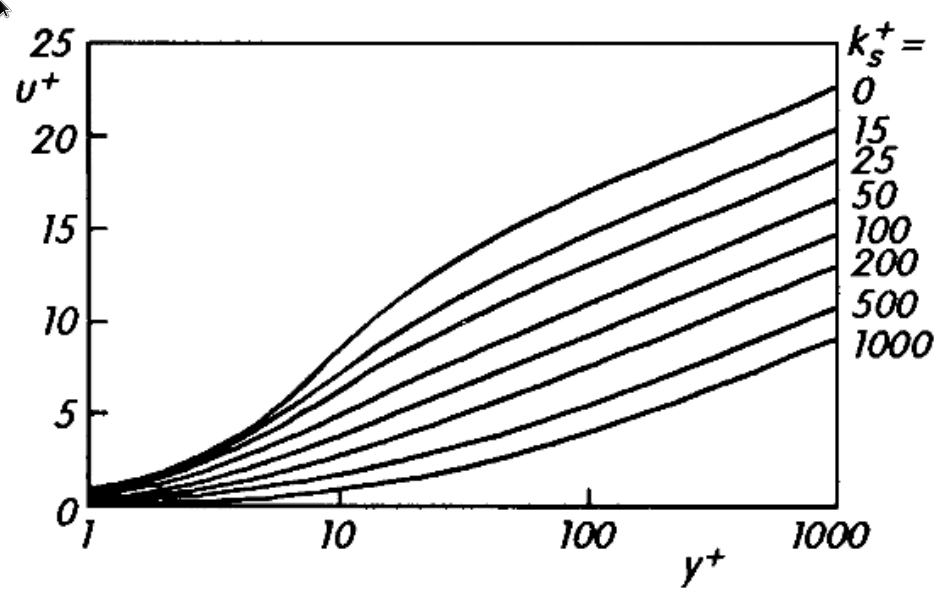
\includegraphics[width=0.4\textwidth]{rough_velocity_dist}
    \caption{Velocity distribution for different surface roughness values \cite{Schlichting2018}.}
    \label{fig:rough_velocity_dist}
\end{figure}


\subsubsection{Rough regimes}
Depending on the height, roughness has different effects on the boundary layer.
It may be classified in tree distinct regimes: \textit{hydraulically smooth},
\textit{transition region} and \textit{fully rough}. They correspond
approximately to the three different regions of the boundary layer. When the
roughness is purely contained by the viscous sublayer, it does not have an
effect at all. When it projects out of the viscous sublayer, the roughness
effect start. If the roughness element projects right into the overlap layer,
the viscosity effects vanish and the flow becomes fully rough
\cite{Schlichting2018}.


When looking at equation \ref{eq:overlap_law}, it simply changes the variable
$C^{+}$. Thus it may be summarized as follows\footnote{Please note $C^{+}$ is
not further described in the transition region.}:

\begin{table}[H]
  \centering
  \begin{tabular}{l l l}
    hydraulically smooth:   & $0 \leq k_{s}^{+} \leq 5$   & $C^{+} \approx 5.0$\\
    transition region:      & $ 5 < k_{s}^{+} < 70$ & $C^{+}(k_{s}^{+})$\\
    fully rough:            & $70 \leq k_{s}^{+}$      & $C^{+} \approx 8.0 - \frac{1}{\kappa} ln(k_{s}^{+})$
  \end{tabular}
  \caption{$C^{+}$ dependence on $k_{s}^{+}$ \cite{Schlichting2018}.}
  \label{tab:opt_prob}
\end{table}

\section{Reynold's Averaged Navier Stokes (RANS)}
The \textit{Navier-Stokes} equations describe how tho the \textit{velocity}
($U$), \textit{pressure} ($P$), \textit{temperature} ($T$) and \textit{density}
($\rho$) of a moving fluid are related. They are differential equations which
almost allway can't be solved analytically. Thus numerical methods are needed.
The physical quantities depend on four variables: \textit{spatial coordinates}
(x, y, z) and the \textit{time} (t). As numerical methods are used, those
quantities need to be discretized \cite{nasaNS}.

In high Reynold's number flows, the length and time-scales of different eddies
differs drastically. To adequately resolve the smallest eddies, which are
basically turbulence, such a fine mesh and timestep would be needed, that it is
not viable. To deal with that, simplifications are needed: (1) solving for a
steady flow and (2) accounting for turbulence stochastically. This means only
one simulation (instead of one every x millisecond) and a much coarser grid is
sufficient.

\subsubsection{Reynolds averaging}
Osborne Reynolds proposed in 1895 a solution which would later be known as
\textit{Reynolds-averaged Navier-Stokes}. The basic idea is to separate the
velocity (and all the other physical properties which are resolved) in two
components \cite{leschziner2015statistical}:

\begin{equation}
  U_{i} = \bar U_{i} + u_{i}^{\prime} \qquad
  P = \bar P + p^{\prime}
\end{equation}

\noindent Where the subscript $i$ stands for all three spatial coordinates (x,
y, z). $\bar U_{i}$ is the mean velocity, which does not change and
$u_{i}^{\prime}$ is the fluctuating part due to turbulence which is not
resolved. The same notation is used for $P$. Plugging this into the
incompressible Navier-Stokes equations leads to:

\begin{equation}
  \label{eq:incomp_RANS}
  \frac{\partial \rho \bar U_{i} \bar U_{j}}{\partial x_{j}} =
  \frac{\partial \bar P}{\partial x_{i}} +
  \frac{\partial}{\partial x_{j}} \nu (\frac{\partial \bar U_{i}}{\partial x_{j}} +
  \frac{\partial \bar U_{j}}{\partial x_{i}}) -
  \frac{\partial}{\partial x_{j}} \rho u_{i}^{\prime} u_{j}^{\prime}
\end{equation}

\noindent Where $\rho u_{i}^{\prime} u_{j}^{\prime}$ are the \textit{six} independent
\textit{Reynolds-stresses} which may be denoted in tensor notation:

\begin{equation}
  \rho \bar u_{i} \bar u_{j} = \rho
  \begin{pmatrix}
    u_{1}^{\prime 2}              & u_{1}^{\prime} u_{2}^{\prime} & u_{1}^{\prime} u_{3}^{\prime} \\
    u_{2}^{\prime} u_{1}^{\prime} & u_{2}^{\prime 2}              & u_{2}^{\prime} u_{3}^{\prime} \\
    u_{3}^{\prime} u_{1}^{\prime} & u_{3}^{\prime} u_{2}^{\prime} & u_{3}^{\prime 2}
  \end{pmatrix}
\end{equation}

\noindent Equation \ref{eq:incomp_RANS} is complemented by the Reynolds-averaged
mass-conservation equation:

\begin{equation}
  \frac{\partial \rho \bar U_{j}}{\partial x_{j}} = 0
\end{equation}


\subsubsection{Turbulence model}
To calculate the unknown Reynolds-stresses, a \textit{turbulence model} is used.
There exist multiple approaches, but two are the most widely used: \textit{Eddy
viscosity models} and \textit{Reynolds stress transport models}. As the
\textit{Spalart Allmaras} model is the former one, only this is explained in more
detail.

\paragraph{Eddy viscosity models}
These kind of models depend on the \textit{Boussinesq-assumption} which says
that the effect of turbulence is similar to that of an increased viscosity. Thus
it introduces the \textit{eddy viscosity} $\mu_{t}$. After some equation
mangling one may calculate the Reynolds stresses from the eddy viscosity as
follows:

\begin{equation}
  - \rho u_{i}^{\prime} u_{j}^{\prime} =
  \nu_{t} (\frac{\partial \bar U_{i}}{\partial x_{j}} +
  \frac{\partial \bar U_{j}}{\partial x_{i}}) -
  \frac{2}{3} \delta_{ij} \rho k
  \label{eq:boussinesq}
\end{equation}

\noindent Where

\begin{align*}
  \delta_{ij} = \; &0 \qquad \text{for} \qquad i \neq j \\
                   &1 \qquad \text{for} \qquad i = j
\end{align*}

\noindent and $k$ is the \textit{turbulent kinetic energy}. Thus the calculation
of the six Reynolds-stresses has reduced to calculating $\nu_{t}$ and $k$
\cite{leschziner2015statistical}.


\subsection{Spalart Allmaras (SA) turbulence model}
The \textit{Spalart Allmaras} turbulence model has been introduced in 1992. It
is a \textit{one-equation} model which means it only computes the eddy viscosity
$\mu_{t}$. When looking at equation \ref{eq:boussinesq}, the most right hand
term is a correction which is neglected as the turbulent kinetic energy is not
readily available. Therefore this model trades accuracy for speed
\cite{leschziner2015statistical} \cite{nasatmr}.

Analog to $u^{+}$ one can convert the eddy viscosity to wall scaling:

\begin{equation}
  \nu_{t}^{+} = \frac{\nu_{t}}{\nu}
\end{equation}

\noindent In figure \ref{fig:nu_t_wall}, its contour is plotted in the boundary
layer of a flat plate a zero incidence. It is almost linear in the logarithmic
region, but varies as $(y^{+})^{4}$ in the viscous sublayer. Finite volume
methods are only able to interpolate linearly in cells. This means a high number
of cells would be needed to properly represent $\nu_{t}^{+}$ in the viscous
sublayer. The Idea of the Spalart Allmaras (SA) turbulence model is to replace
$\nu_{t}^{+}$ with a modified eddy viscosity $\tilde \nu^{+}$ which behaves
linearly right to the surface. Additionally to reducing the number of cells,
this also makes the numerical behavior more stable. As the viscous sublayer can
not be neglected, the SA model adjusts $\tilde \nu^{+}$ in a post-processing step
to reflect the real $\nu_{t}^{+}$ behavior \cite{KALITZIN2005265} \cite{fluid_101}.

\begin{figure}[H] \centering
  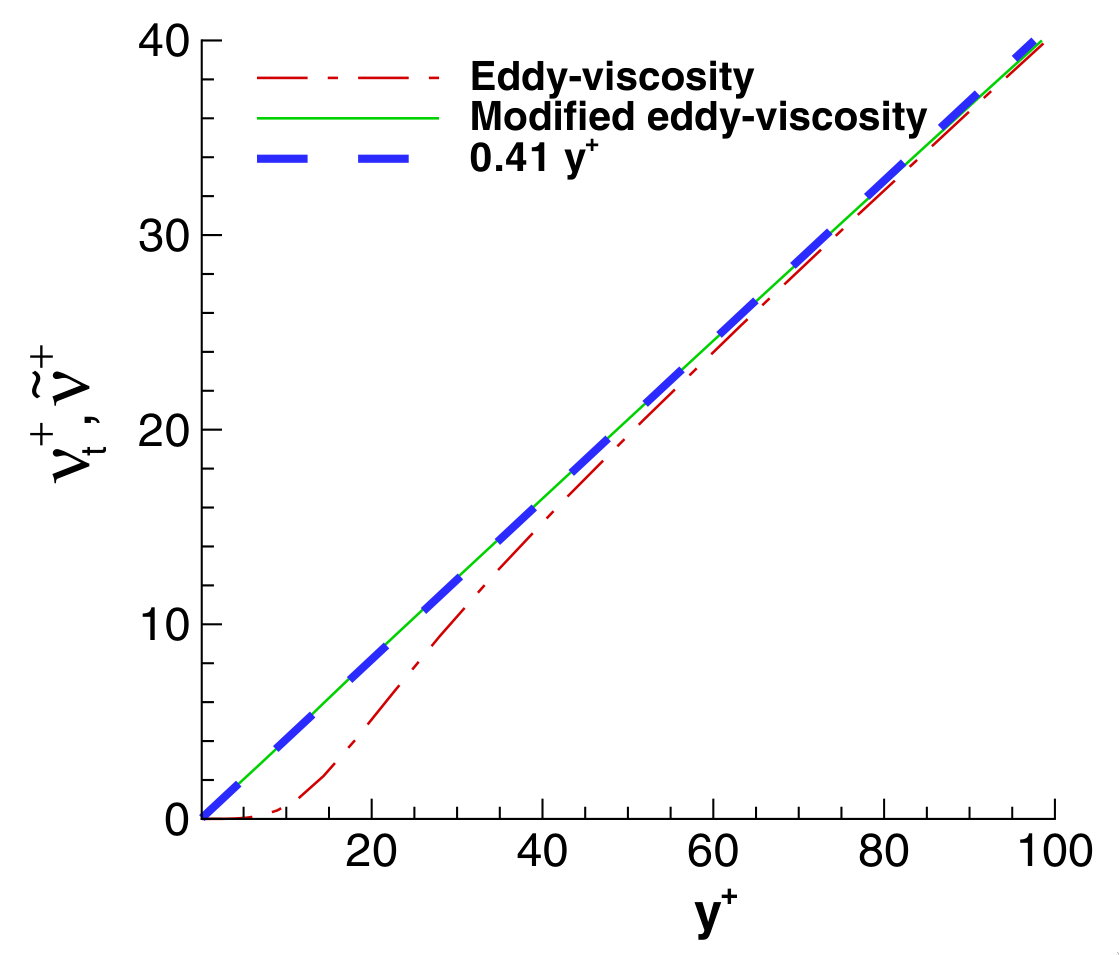
\includegraphics[width=0.5\textwidth]{eddy_viscosity}
  \caption{Eddy viscosity $\nu_{t}^{+}$ and modified eddy viscosity
    $\tilde \nu^{+}$ used in the Spalart Allmaras model \cite{KALITZIN2005265}.}
  \label{fig:nu_t_wall}
\end{figure}

\noindent The transport equation is given by \cite{nasatmr}:

\begin{equation}
  \frac{D \tilde \nu}{D t} =
  c_{b1}(1 - f_{t2}) \tilde S \tilde \nu -
  \left[ c_{w1}f_{w} - \frac{c_{b1}}{\kappa^{2}}f_{t2} \right]
  \left( \frac{\tilde \nu}{d} \right) ^{2} +
  \frac{1}{\sigma} \left[ \frac{\partial}{\partial x_{j}}
  \left( (\nu + \tilde \nu) \frac{\partial \tilde \nu}{\partial x_{j}}\right) +
  c_{b2} \frac{\partial \tilde \nu}{\partial x_{i}} \frac{\partial \tilde \nu}{\partial x_{i}} \right]
\end{equation}

\noindent Then, the turbulent energy is computed as:

\begin{equation}
  \nu_{t} = \rho \tilde \nu f_{v1}
\end{equation}

\noindent where

\begin{align}
  f_{v1} &= \frac{\chi^{3}}{\chi^{3} + c_{v1}^{3}} &
  \chi &= \frac{\tilde \nu}{\nu} &
  \tilde S &= \Omega + \frac{\tilde \nu}{\kappa^{2} d^{2}} f_{v2} \\
  \Omega &= \sqrt{2W_{ij}W_{ij}} &
  f_{v2} &= 1 - \frac{\chi}{1 + \chi f_{v1}} &
  f_{w} &= g \left[ \frac{1 + c_{w3}^{6}}{g^{6} + c_{w3}^{6}} \right] ^{1/6} \\
  g &= r + c_{w2}(r^{6} -r) &
  r &= min \left[ \frac{\tilde \nu}{\tilde S \kappa^{2} d^{2}} \right] &
  f_{t2} &= c_{t3} exp(-c_{t4} \chi^{2}) \\
  W_{ij} &= \frac{1}{2} \left( \frac{\partial u_{i}}{x_{j}} - \frac{\partial u_{j}}{\partial x_{i}}\right) &
  d &= \text{Distance to the nearest wall}
\end{align}

\noindent The boundary conditions are:
\begin{equation}
  \tilde \nu_{wall} = 0
  \qquad \qquad
  \tilde \nu_{farfield} = 3\nu_{\infty} :to: 5\nu_{\infty}
\end{equation}

\noindent And the constants are:
\begin{align*}
  c_{b1} &= 0.1355 &
  \sigma &= 2/3 &
  c_{b2} &= 0.622 &
  c_{w1} &= \frac{c_{b1}}{\kappa^{2}} + \frac{1 + c_{b2}}{\sigma} \\
  c_{w2} &= 0.3 &
  c_{w3} &= 2 &
  c_{v1} &= 7.1 &
  c_{t3} &= 1.2 \\
  c_{t4} &= 0.5
\end{align*}

\noindent Please note the distance to the nearest wall $d$ is used as the
turbulence length scale. It reduces the size of the eddies near the wall. This
is a physical phenomenon which has been observed in reality
\cite{leschziner2015statistical}. But it can be a challenge for parallel
CFD-codes as those distances must be communicated across different processors.


\subsection{Modification of SA for rough walls}
\label{subsec:mod_sa_rough}
As can bee seen in figure \ref{fig:rough_velocity_dist}, the main effect of
roughness is a downward shift in the log region. According to \cite{sa_rough},
two different methods are proposed:

\begin{itemize}
  \item Models where the eddy viscosity is zero at the wall. The effect of the
        roughness is modeled through a reduction of the damping function.
  \item Models where the eddy viscosity is not zero at wall. This can be
        interpreted as shifting the wall upwards into the roughness.
        Apparently, this approach works better for small roughness values.
\end{itemize}

\noindent There exists two different extension for the SA model which employ the
strategy of a non zero eddy viscosity at the wall. One proposed by
\textit{Boeing} and the other by \textit{ONERA}. The approach by ONERA is
slightly more complicated\footnote{It changes the SA model more.} and also needs
the friction velocity. Thus this work implemented the extension proposed by
Boeing.

\subsubsection{Changed terms}
The biggest change is the distance $d$ which accounts for the shift of a
'virtual' wall upwards \cite{sa_rough}\cite{nasatmr}:

\begin{equation}
  \label{eq:d_new}
  d_{new} = d + 0.03k_{s}
\end{equation}

\noindent Additionally, $\chi$ is modified:

\begin{equation}
  \label{eq:chi_new}
  \chi = \frac{\tilde \nu}{\nu} + c_{R1} \frac{k_{s}}{d_{new}}
\end{equation}

\noindent Where

\begin{equation*}
  c_{R1} = 0.5
\end{equation*}

\noindent As the new definition of $\chi$ should not affect $\tilde S$, the
function $f_{v2}$ also needs to be modified:

\begin{equation}
  \label{eq:fv2_new}
  f_{v2} = 1 - \frac{\tilde \nu}{\nu + \tilde \nu f_{v1}}
\end{equation}

\noindent And finally, the boundary condition is replaced by:

\begin{equation}
  \left( \frac{\partial \tilde \nu}{\partial n} \right)_{wall} =
  \frac{\tilde \nu_{wall}}{0.03k_s}
\end{equation}



\section{Adjoint method}
Please refer to the report of the \textit{complementary module 1} for more
information about the adjoint method \cite{cm1}.
